\documentclass[12pt,a5paper]{book}
\usepackage[utf8]{vietnam}
\usepackage{amsmath}
\usepackage{amsfonts}
\usepackage{tikz}
\usepackage{amssymb}
\usepackage{graphicx}
\usepackage{listings}
\usepackage{textcomp}
\usepackage[hidelinks]{hyperref}

\renewcommand{\familydefault}{\sfdefault}
\usepackage[left=2cm,right=1.5cm,top=1.5cm,bottom=1.5cm]{geometry}

 \renewcommand\lstlistingname{Quelltext} % Change language of section name

\lstset{ % General setup for the package
	language=C,
	basicstyle=\small\sffamily,
	numbers=left,
 	numberstyle=\tiny,
	frame=tb,
	tabsize=4,
	columns=fixed,
	showstringspaces=false,
	showtabs=false,
	keepspaces,
	%commentstyle=\color{green},
	%keywordstyle=\color{blue}
}
\pagenumbering{gobble}
\pagenumbering{arabic}
\title{LẬP TRÌNH NHÚNG}
\author{Nguyễn Thành Công}


\begin{document}
\maketitle
\begin{figure}
\centering
 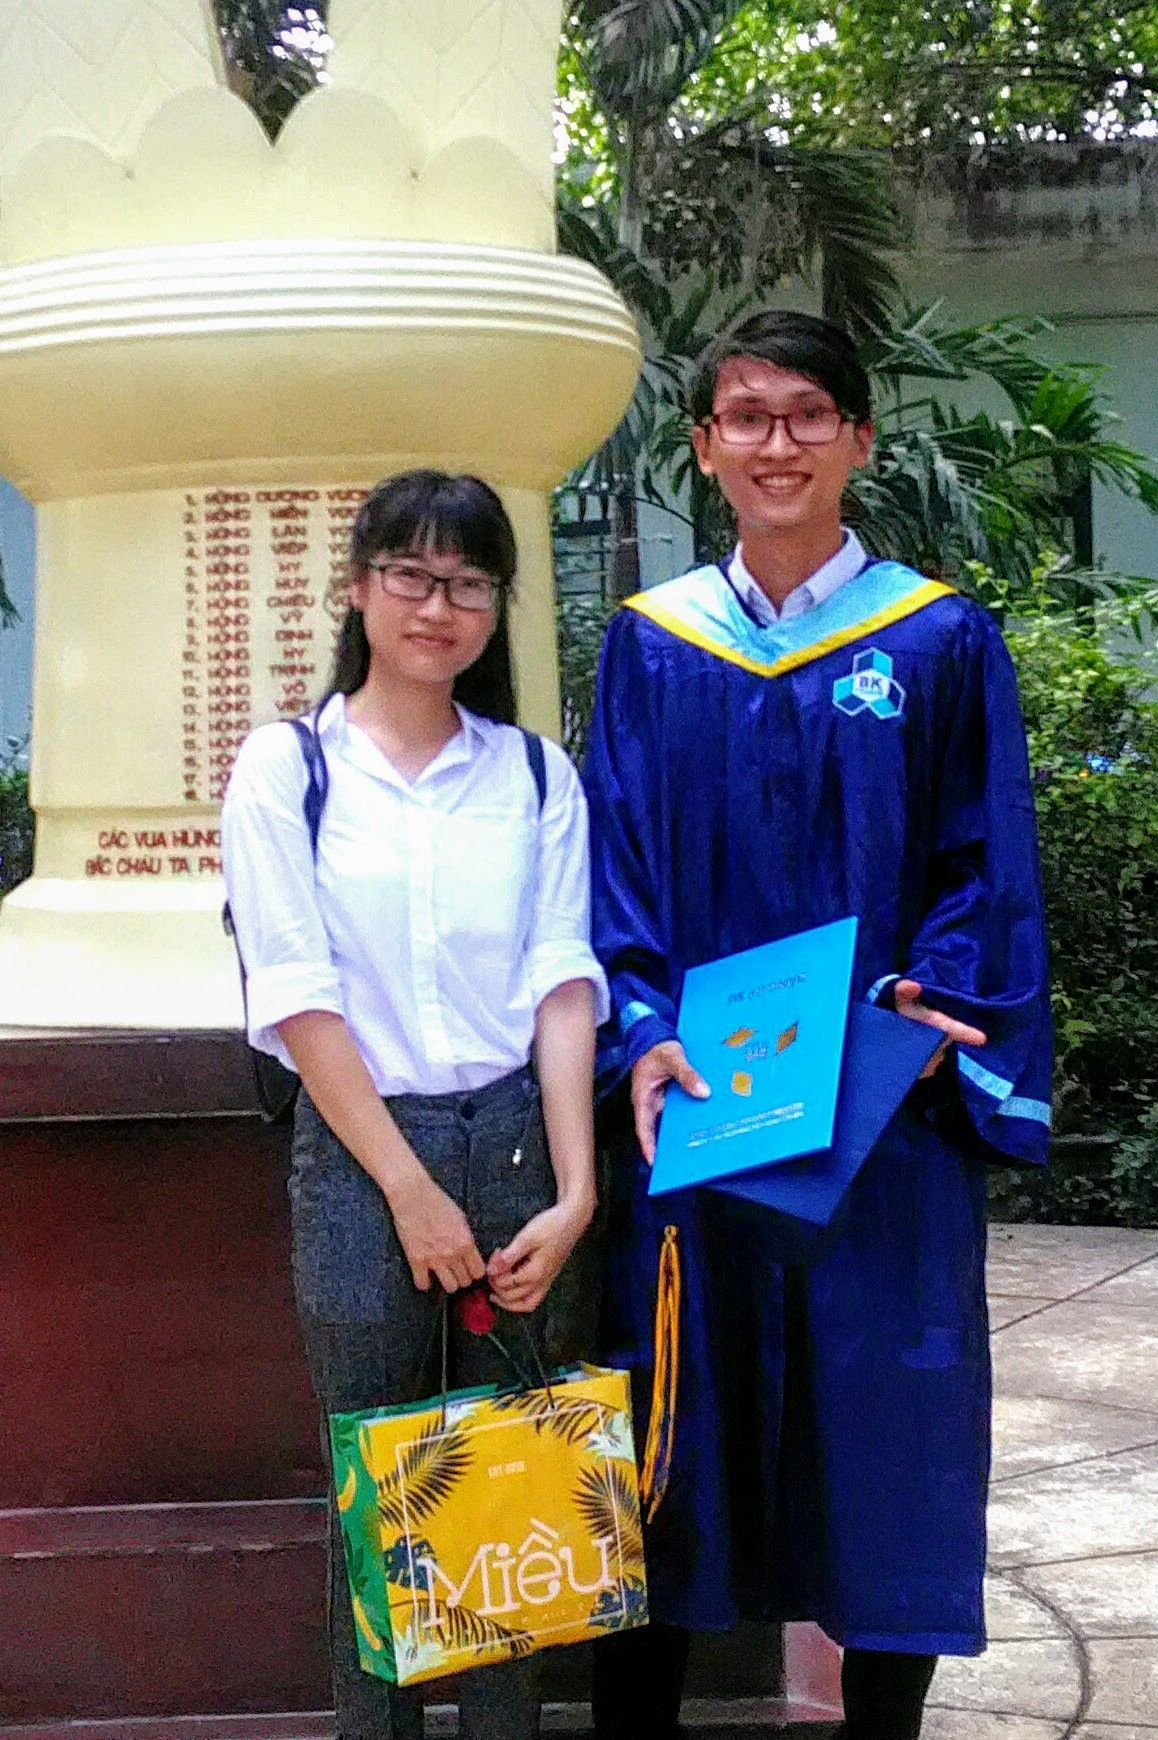
\includegraphics[width=0.5\linewidth]{tao.jpg}
 \caption{Tui}
\end{figure}
\tableofcontents{}
 \chapter{Chém gió xíu }
	\section{Về lập trình nhúng}
		\paragraph{}
Đặc trưng của lập trình nhúng là viết chương trình để điều khiển phần cứng, ví dụ như chương trình điều khiển động cơ bước chẳng hạn. Với phần mềm ứng dụng như trên máy tính mà phần cứng yêu cầu giống nhau (màn hình, chuột, cpu...) và đòi hỏi nặng về khả năng tính toán của cpu. Còn với chương trình nhúng thì phần cứng của nó cực kì đa dạng, khác nhau với mỗi ứng dụng như chương trình điều khiển động cơ hoặc chương trình đọc cảm biến, nó không đòi hỏi cpu phải tính toán quá nhiều, chỉ cần quản lý tốt phần cứng bên dưới. 
		\paragraph{}
Có 2 khái niệm là Firmware, ý chỉ chương trình nhúng, và Software, chương trình ứng dụng trên máy tính, được đưa ra để người lập trình dễ hình dung, nhưng không cần thiết phải phân biệt rõ ràng.
		\paragraph{}
Khi lập trình hệ thống nhúng, việc biết rõ về phần cứng là điều cần thiết. Bởi bạn phải biết phần cứng của mình như thế nào thì bạn mới điều khiển hoặc quản lí tốt nó được. Tốt nhất là làm trong team hardware một thời gian rồi nhảy qua team firmware, hoặc làm song song cả hai bên (nếu bạn đủ sức).
		\paragraph{}
Tóm lại: \textit{Lập trình nhúng là viết chương trình điều khiển phần cứng, bạn phải biết lập trình, và phải giỏi về phần cứng.} 
	\section{Về ngôn ngữ C trong lập trình nhúng}
		\paragraph{}
	Ngôn ngữ C cho phép tương tác rất mạnh tới phần cứng, mạnh thế nào thì hồi sau sẽ rõ, thế nên nó thường được lựa chọn trong các dự án lâp trình nhúng. Ngoài ra có thể dùng C++ và Java nhưng mình ít xài chúng nên không đề cập ở đây.
		\paragraph{}
	Việc học C cơ bản mình sẽ không đề cập tới vì tài liệu nó nhiều lắm, các bạn có để xem và làm vài bài tập sử dụng được ngôn ngữ này. Lưu ý là ranh giới giữa việc \textbf{biết} và \textbf{sử dụng được} ngôn ngữ C là việc bạn có làm bài tập hay không nhé. Về cú pháp thì nó quanh đi quẩn lại chỉ là khai báo biến, rồi mấy vòng lặp for, while hoặc rẽ nhánh if, else chẳng hạn, nhưng \textbf{kỹ năng} sử dụng C để giải quyết một vấn đề thì cần nhiều bài tập để trau dồi.
		\paragraph{}
	Tóm lại: \textit{bạn không thể đọc sách học bơi là biết bơi, không thể đọc kiếm phổ là thành cao thủ.}
	\section{Về phần cứng để demo}
	\paragraph{}
	Trong phần này mình sẽ sử dụng kit STM32F4 Discovery để thực hành, phần mềm KeilC v5 để code cho nó. Bạn nên mua một cái kit, học cách sử dụng STM32CubeMX và làm quen với thư viện HAL (trên youtube có kênh Học ARM hướng dẫn khá đầy đủ phần này). Mà nói trước là việc tự học là rất quan trọng. Bạn có thể được dạy một vài loại phần cứng như tiva, 8051 hoặc pic nhưng không có nghĩa là bạn phải xài cái đó hoài. Bạn có thể dùng bất cứ loại nào nếu chịu tìm hiểu. Ngoài ra phần thiên về lập trình không cần phần cứng sẽ sử dụng chương trình DevC++ (nhớ tạo project C, không cần C++), những cái cơ bản các bạn nên tự tìm hiểu nhé, vì những cái đó tài liệu nó rất nhiều, và bạn cũng có thể tự mò cho quen.
	\section{Về Tiếng Anh, vâng tiếng Anh...}
		\paragraph{}
	Mấy ngành khác thì mình không rành chứ mà làm nhúng mà bạn không biết Tiếng Anh là tự níu chân mình lại. Vì mỗi linh kiện điện tử đều kèm theo một cái bảng thông tin đặc tính là datasheet, cái nào phức tạp thì sẽ kèm theo một cái hướng dẫn sử dụng là user manual. Và tất nhiên 96.69\% chúng được viết bằng tiếng Anh, còn lại là tiếng Trung Quốc. Và tin buồn là code trong lập trình nhúng đều biết bằng tiếng Anh, tin buồn hơn nữa là tài liệu, sách hướng dẫn, các diễn đàn sử dụng tiếng Anh rất nhiều và nhiều cái rất hay.
		\paragraph{}
	Tóm lại là không biết nó thì công việc của bạn bị cản trở rất nhiều, phụ thuộc rất nhiều vào google dịch củ chuối. Hãy dừng một bước để học tiếng anh và tiến 3 bước trong con đường sự nghiệp. Chí ít bạn phải đọc được datasheet mà không cần tra quá nhiều từ, đọc được cuốn sách như clean code chẳng hạn, hoặc viết email cho thằng bán linh kiện ở Trung Quốc vì kiểu gì sau này bạn cũng đặt hàng ở bên đó.
		\paragraph{}
	\textit{Nhớ rằng tiếng Anh là công cụ để sử dụng. Như người ta học đi xe máy để đi lại nhanh hơn. Hãy học tiếng Anh để làm việc ngon lành hơn.}


	\chapter{Ngôn ngữ C trong lập trình nhúng}
	\paragraph{}
Hãy nhớ là bạn làm vài bài tập về ngôn ngữ C rồi hãy đọc phần này nhé.
	\paragraph{}
Có cuốn sách hay mà bạn có thể kiếm là Nhập Môn Lập Trình của trường Khoa Học Tự Nhiên (sách bìa màu đen ấy).\\
	\section{Cơ bản về chương trình.}
	\paragraph{} 
Đại khái thì việc lập trình là chỉ cho cái máy biết bạn muốn nó làm cái gì.
	\paragraph{}
Khi bạn viết chương trình, bên dịch thì máy tính sẽ biên dịch code của bạn (người hiểu được) thành mã máy (máy hiểu được) bao gồm các lệnh mà vi điều khiển sẽ thực và khi nạp xuống cho vi điều khiển thì chương trình sẽ được lưu ở ROM (bộ nhớ chương trình). CPU sẽ đọc lệnh từ bộ nhớ chương trình rồi thực thi. Lưu ý là CPU chỉ đọc thôi nhé, nó không được phép ghi gì vào bộ nhớ chương trình. Nó không thể cãi lệnh bạn! Thế nên bộ nhớ chương trình có tên là bộ nhớ chỉ đọc (Read-only memory, ROM). Nó vẫn còn đấy khi mất điện.
	\paragraph{}
Còn bộ nhớ RAM là để phục vụ cho chương trình được thực thi.
	\paragraph{}
Ví dụ như bạn khai báo biến int a=0; thì biến a sẽ được lưu trong RAM. Sau đó có lệnh a=a+1; CPU sẽ lấy biến a từ trong RAM ra, thực hiện phép tính rồi lại lưu vào chỗ cũ.
	\paragraph{}
Do việc RAM được CPU sử dụng để thực hiện chương trình, đọc ghi liên tục nên nó gọi là bộ nhớ truy cập ngẫu nhiên (Random-access Memory) hay nói cách khác CPU đươc toàn quyền sử dụng bộ nhớ RAM (không như việc chỉ được quyền đọc từ ROM thôi nhé).



	\section{Về cách tổ chức bộ nhớ}
	\paragraph{}
	Thông thường thì đơn vị nhỏ nhất của bộ nhớ là byte (mà mình hay gọi là ô nhớ), mỗi byte đươc đánh một địa chỉ. Nếu vi xử lý 8-bit thì nó có thể quản lý 256 byte bộ nhớ, vi xử lý 16-bit thì có thể quản lý 64kbyte, còn 32-bit thì có thể quản lý tới 4Gbyte bộ nhớ. 
	
\begin{figure}[h!]
	\centering
	
	%\label{fig:Bộ nhớ 16 bit}
	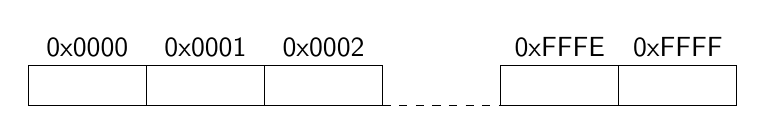
\begin{tikzpicture}[yscale=0.5, xscale=1.5]

		\draw (0,0) rectangle (1,1);
		\draw (1,0) rectangle (2,1);
		\draw (2,0) rectangle (3,1);
		\draw [dashed] (3,0) -- (4,0);
		\draw (4,0) rectangle (5,1);
		\draw (5,0) rectangle (6,1);
		\node  [above] at (0.5, 1) {0x0000};
		\node  [above] at (1.5, 1) {0x0001};
		\node  [above] at (2.5, 1) {0x0002};
		\node  [above] at (4.5, 1) {0xFFFE};
		\node  [above] at (5.5, 1) {0xFFFF};
	\end{tikzpicture}
	\caption{Bộ nhớ địa chỉ 16-bit} 
\end{figure}

	Vậy mỗi ô nhớ sẽ có 2 thông số mà bạn cần quan tâm: địa chỉ (nó ở đâu, địa chỉ có thể là số 8-bit, 16-bit, 32-bit...), và giá trị được lưu (nó bao nhiêu, chỉ là số 8-bit (1 byte) thôi).
	
	\begin{figure}[h!]
	\centering
	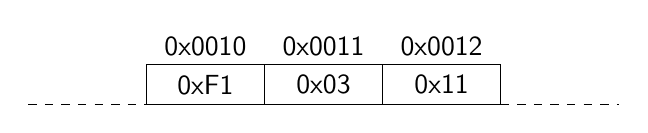
\begin{tikzpicture}[yscale=0.5, xscale=1.5]
		\draw [dashed] (0,0) -- (1,0);
		\draw (1,0) rectangle (2,1);
		\draw (2,0) rectangle (3,1);
		\draw (3,0) rectangle (4,1);
		\draw [dashed] (4,0) -- (5,0);
		
		\node  [above] at (1.5, 1) {0x0010};
		\node  [above] at (2.5, 1) {0x0011};
		\node  [above] at (3.5, 1) {0x0012};
		\node   at (1.5, 0.5) {0xF1};
		\node   at (2.5, 0.5) {0x03};
		\node   at (3.5, 0.5) {0x11};

	\end{tikzpicture}
	\caption{Dữ liệu trong bộ nhớ} %\label{fig: Dữ liệu trong bộ nhớ}
\end{figure}

	\paragraph{}
	Chip STM32 là vi điều khiển 32-bit nhưng nó chỉ có vài kbyte bộ nhớ RAM nên dãy địa chỉ RAM có thể được đánh dấu từ 0x00000000 đến 0x0000FFFF chẳng hạn. Nếu bạn muốn ghi vào địa chỉ 0xF0000000 thì nó sẽ biến mất hoặc báo lỗi không biết trước được.
	\paragraph{}
	Đoạn chương trình để xem địa chỉ trong DevC++:\*
\begin{lstlisting}
	#include <stdio.h>
	void main(){
		char a;
		printf("a address: 0x%08x\n", &a);
	}
\end{lstlisting}

	
	\section{Khai báo biến}
	\paragraph{}
Các kiểu biến thông thường khi lập trình C là char, int, long, float double. Nhưng trong lập trình nhúng, tài nguyên bộ nhớ hạn chế nên việc bạn biết các biến chiếm bao nhiêu ô nhớ là điều rất quan trọng. Thông thường, các biến được khai báo dưới dạng uint8\_t, int8\_t, uint16\_t, int16\_t... để sử dụng thì bạn cần  \#include <stdint.h>. Đoán xem mỗi kiểu sẽ chiếm bao nhiêu ô nhớ, và kiểu nào là kiểu có dấu, không đấu?
	\paragraph{}
	Một điểm đặc biệt là kiểu uint8\_t thường được dùng để đại diện cho một ô nhớ (8-bit). Ví dụ khi khai báo uint8\_t array[3], thì có thể hiểu là khai báo 3 phần tử mảng array có kiểu là uint8\_t, hoặc cũng có thể hiểu là yêu cầu bộ nhớ cấp 3 ô nhớ kề nhau. Việc này thường được dùng để khai báo các bộ đệm trong các giao tiếp như uart, i2c, spi...
	\paragraph{}
	Thế nên hãy thường sử dụng các kiểu dữ liệu với bộ nhớ tường minh trên để kiểm soát bộ nhớ chặt chẽ hơn.\\
\section{Kiểu dữ liệu tự định nghĩa}
\paragraph{}
Ngôn ngữ C cung cấp cơ chế tự định nghĩa kiểu dữ liệu để việc truy xuất dữ liệu được thuận tiện.

\paragraph{}
Ví dụ mình có một cái cảm biến có thể đọc về nhiệt độ, độ ẩm và ánh sáng môi trường. Dữ liệu nhiệt độ từ  -20\textdegree{}C đến 100\textdegree{}C, độ ẩm từ 0\% đến 100\%, ánh sáng từ 0 lux đến 50.000 lux. Vậy mình khai báo dữ kiểu dữ liệu env\_t (environment type) như sau: 
\begin{lstlisting}
	typedef struct{
		int8_t temp;
		uint8_t humi;
		uint16_t lux;
	}env_t;
\end{lstlisting}
\paragraph{}
Dễ thấy là các kiểu biến bên trong đều chứa đủ khoảng giá trị cần thiết (nếu nhiệt độ vượt quá 127\textdegree{}C thì biến int8\_t không chứa được, phải chọn kiểu khác).
\paragraph{}
Thực chất kiểu dữ liệu là cách bạn tương tác với một vùng nhớ cho trước. Ví dụ khi khai báo một biến như \textit{env\_t evn;} chẳng hạn, nó sẽ cung cấp cho bạn 4 ô nhớ liền nhau. Nếu bạn in địa chỉ của biến env ra nó sẽ hiển thị địa chỉ ô nhớ \textbf{đầu tiên} của dãy 4 ô nhớ đó. Và kiểu env\_t sẽ cho máy tính biết cách truy cập tới 4 ô nhớ đó như thế nào.

\begin{figure}[h!]
	\centering
	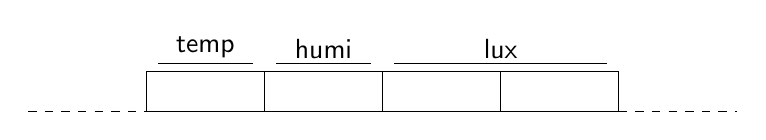
\begin{tikzpicture}[yscale=0.5, xscale=1.5]
		\draw [dashed] (0,0) -- (1,0);
		\draw (1,0) rectangle (2,1);
		\draw (2,0) rectangle (3,1);
		\draw (3,0) rectangle (4,1);
		\draw (4,0) rectangle (5,1);
		\draw [dashed] (5,0) -- (6,0);
		
		\draw (1.1, 1.2) -- (1.9, 1.2);
		\node [above] at (1.5, 1.1) {temp};
		
		\draw (2.1, 1.2) -- (2.9, 1.2);
		\node [above] at (2.5, 1.1) {humi};
		
		\draw (3.1, 1.2) -- (4.9, 1.2);
		\node [above] at (4, 1.1) {lux};
		
	\end{tikzpicture}
	\caption{Truy cập biến kiểu env\_t} %\label{fig: Dữ liệu trong bộ nhớ}
\end{figure}
\paragraph{}
Đoạn chương trình xem độ dài của kiểu dữ liệu:
\begin{lstlisting}
#include <stdio.h>
#include <stdint.h>

typedef struct{
	int8_t temp;
	uint8_t humi;
	uint16_t lux;
}env_t;

void main(void) {
	printf("Size of env_t: %d\n", sizeof(env_t));
}
\end{lstlisting}
\paragraph{}
Một điểm cần lưu ý là các máy tính thường có cơ chế làm tròn biên kiểu dữ liệu (data structure alignment). Nếu chúng ta khai báo như sau:

\begin{lstlisting}
typedef struct{
	int8_t temp;
	uint16_t lux;
	uint8_t humi;
}env_t;
\end{lstlisting}
biến lux khai báo ở giữa, thì kiểu dữ liệu env\_t giờ đây có độ dài là 6 byte chứ không phải 4!!!.
\paragraph{}
Kiểu biến env\_t giờ có cấu trúc như sau:
\begin{figure}[h!]
	\centering
	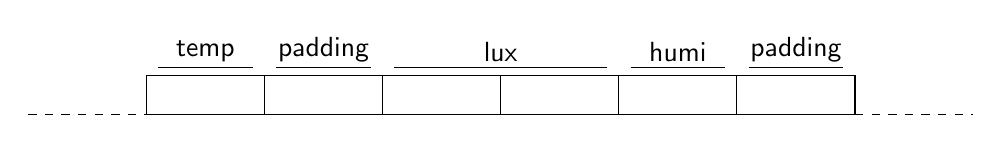
\begin{tikzpicture}[yscale=0.5, xscale=1.5]
		\draw [dashed] (0,0) -- (1,0);
		\draw (1,0) rectangle (2,1);
		\draw (2,0) rectangle (3,1);
		\draw (3,0) rectangle (4,1);
		\draw (4,0) rectangle (5,1);
		\draw (5,0) rectangle (6,1);
		\draw (6,0) rectangle (7,1);
		\draw [dashed] (7,0) -- (8,0);
		
		\draw (1.1, 1.2) -- (1.9, 1.2);
		\node [above] at (1.5, 1.1) {temp};
		
		\draw (2.1, 1.2) -- (2.9, 1.2);
		\node [above] at (2.5, 1.1) {padding};
		
		\draw (3.1, 1.2) -- (4.9, 1.2);
		\node [above] at (4, 1.1) {lux};
		
		\draw (5.1, 1.2) -- (5.9, 1.2);
		\node [above] at (5.5, 1.1) {humi};
		
		\draw (6.1, 1.2) -- (6.9, 1.2);
		\node [above] at (6.5, 1.1) {padding};
	\end{tikzpicture}
	\caption{Truy cập biến kiểu env\_t} 
\end{figure}
\paragraph{}
Hai ô nhớ tên padding được thêm vào để tăng hiệu suất việc đọc ghi dữ liệu trong máy tính hiện đại. Các bạn quan tâm thì có thể tìm hiểu thêm. Ta có thể tránh nó bằng cách khai báo như sau: trong DevC++ thì bạn khai báo \textit{\#pragma pack(1)} trước khi khai báo biến dữ liệu, còn trong KeilC thì khai báo kiểu:

\begin{lstlisting}
typedef __packed struct{
	int8_t temp;
	uint16_t lux;
	uint8_t humi;
}env_t;
\end{lstlisting}
mỗi khi khai báo một kiểu biến nào đó.

\paragraph{}
Ngoài ra còn một số kiểu enum và union mà các bạn hỏi giáo sư gu gồ hen.

\section{Con trỏ}
\paragraph{}
Có thể nói con trỏ là công cụ lợi hại nhất của C, bạn khó mà giỏi C nếu bỏ qua con trỏ được. Bản chất của con trỏ (chưa nói đến con trỏ hàm) là trỏ tới một vùng nhớ nào đó và tương tác với vùng nhớ đó. Chương trình ví dụ về con trỏ:
\begin{lstlisting}
#include <stdio.h>
#include <stdint.h>

int main(void) {
	uint16_t a=0;
	uint16_t *pa;
	pa=&a;
	printf("a addr: 0x%08x\n", &a);
	printf("a addr: 0x%08x\n", pa);
}
\end{lstlisting}

hai lần printf sẽ cho ra kết quả như nhau vì đã gán địa chỉ của a cho pa.
\paragraph{}
Lưu ý là bạn không cần quan tâm địa chỉ thật của a (có dạng số hex như 0x0012) chỉ cần khai báo biến a, nó sẽ nằm đâu đó trong RAM (nếu RAM còn trống) và có phép lấy địa chỉ \&a.
\paragraph{}
Một con trỏ cần 2 thông tin sau để có thể hoạt động được: địa chỉ và kiểu dữ liệu nó sẽ trỏ tới. Như chương trình trên thì dòng số 6 sẽ cấp cho con trỏ kiểu dữ liệu, dòng số 7 cấp địa chỉ. 2 yếu tố trên giúp bạn có thể đi đến vùng nhớ mà bạn quan tâm sau đó có thể truy cập vùng nhớ đó theo cách bạn muốn.
\paragraph{}
Một lưu ý là ngôn ngữ C đồng nhất giữa mảng và con trỏ. Ví dụ mình khai báo mảng uint32\_t arr[4], thì \textit{arr} là địa chỉ của phần tử đầu tiên của mảng, hay arr=\&arr[0] (cùng 1 địa chỉ), *arr=arr[0] (cùng 1 giá trị). Giả sử arr là địa chỉ 0x0010 thì arr+1 sẽ là địa chỉ của arr[1] có địa chỉ là 0x0014 (không phải 0x0011 he, đo mỗi biến có 4 ô nhớ, kiểm tra lại bằng DevC++).
\section{Ví dụ về truyền nhận uart}

\paragraph{}
Để biết con trỏ nó lợi hại như thế nào thì các bạn hãy xem ví dụ về truyền nhận uart. Trước khi vào phần này bạn nên tham khảo ví dụ về truyền nhận uart cho kit stm32f4 trên kênh youtube của Học ARM để biết sơ sơ về nó thế nào.
\paragraph{}
Các hàm truyền nhận dữ liệu uart thường có cấu trúc như sau:
\begin{lstlisting}
uart_transmit(uint8_t *data, uint16_t size);
uart_receive(uint8_t *data, uint16_t size);
\end{lstlisting}
\paragraph{}
Trong hàm uart\_transmit, tham số *data là ô nhớ đầu tiên trong chuỗi ô nhớ liên tiếp mà bạn muốn gửi đi. Còn trong hàm uart\_receive, tham số *data là ô nhớ đầu tiên của vùng nhớ mà bạn sẽ cất dữ liệu nhận được vào đấy (địa chỉ bộ đệm).
\subsection{Truyền uart}
\paragraph{}
Mình ví dụ chương trình sau: một MCU đọc cảm biến môi trường, lưu vào biến env (khai báo ở trên), rồi truyền qua đường uart về một MCU khác để xử lý (các bạn làm mấy cái IOT hay gặp cái này).

\paragraph{}
Vậy giờ mình cần gửi một biến env (khi đã nhập dữ liệu cho biến này) đi thì cần làm thế nào để hàm truyền kia có thể truyền một kiểu env\_t đi trong khi hàm truyền nhận uart chỉ nhận vào là kiểu uint8\_t?
\paragraph{}
Cách giải quyết của mình là thế này, tạo một con trỏ kiểu uint8\_t và cấp cho nó địa chỉ của biến env.
\begin{lstlisting}
env_t evn; //env.temp=10; env.humi=70, env.lux=1000;
uint8_t *pe;
pe=(uint8_t *)&evn;
uart_transmit(pe, sizeof(env_t));
\end{lstlisting}
\paragraph{}
Câu lệnh dòng số 4, \textit{pe=(uint8\_t *)\&evn} có 2 phần: đầu tiên là \&evn, lấy địa chỉ của biến env tạo thành một con trỏ tạm thời kiểu evn\_t, sau đó ép kiểu con trỏ (uint8\_t *) này thành uint8\_t và gán cho pe. Vậy pe là một con trỏ kiểu uint8\_t và có địa chỉ của biến env, sau đó mình dùng hàm uart truyền đi 4 ô nhớ bắt đầu từ ô nhớ này. Mấy bạn chưa quen thì nên ngâm cứu kĩ chỗ này nhé :)))
\paragraph{}
Khi sử dụng đến con trỏ, bạn cần có \textbf{tư duy ở ô nhớ} (chứ không phải kiểu dữ liệu) thì việc sử dụng con trỏ sẽ đơn giản hơn rất nhiều. Ví dụ như trong hàm truyền uart, với kiểu uint8\_t đại diện cho ô nhớ, và hai tham số *data và size, có ý nói là hãy đưa tôi địa chỉ ô nhớ đầu tiên và số lượng cần truyền, tôi sẽ truyền cái đống đó đi cho bạn.
\subsection{Nhận uart}
\paragraph{}
Phía nhận muốn nhận được dữ liệu thì trước tiên phải khai báo một bộ đệm, sau đó gọi hàm uart\_receive() trỏ tới bộ đệm này và chờ dữ liệu đến.
\begin{lstlisting}
#define MAX_BUFF 10
uint8_t uart_buffer[MAX_BUFF];
uart_receive(uart_buffer, sizeof(env_t));
\end{lstlisting}
\paragraph{}
Lưu ý là số lượng ô nhớ của bộ đệm phải lớn hớn hoặc bằng số lượng trong một lần truyền, nếu không chương trình sẽ lỗi. Câu lệnh số 1 để định nghĩa số lượng và để lên trên cùng của trang để sau này sửa lại số lượng cho phù hợp (cỡ như chương trình của bạn 1000 dòng mà nhét thẳng số 10 vô khai báo mảng luôn mai mốt tìm lại đuối).
\paragraph{}
Rồi, sau khi nhận được dữ liệu, việc của bạn là đọc dữ liệu và hiển thị lên màn hình lcd hoặc cất đâu đó. Ta tiến hành ép kiểu một lần nữa.
\begin{lstlisting}
env_t *p_env;
p_env = (env_t *)uart_buffer;
printf("Temperature: %d\n", p_env->temp);
printf("Humidity: %d\n", p_env->humi);
printf("Lux: %d\n", p_env->lux);
\end{lstlisting}
\paragraph{}
Như vậy là cùng nhiêu đó ô nhớ nhưng \textbf{cách nhìn các ô nhớ đó} khác nhau với những kiểu dữ liệu khác nhau. Việc ép kiểu không làm thay đổi nội dung của ô nhớ vật lý (nó vẫn là cái đống 00 11 đó thôi), nhưng nó thay đổi cách bạn đọc nó.
\begin{figure}[h!]
	\centering
	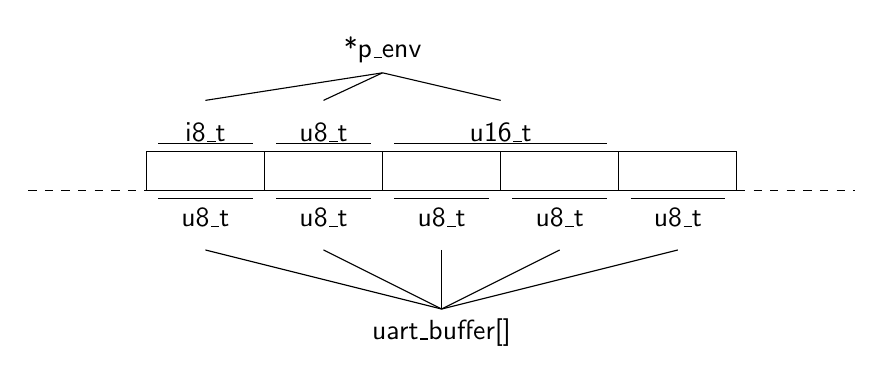
\begin{tikzpicture}[yscale=0.5, xscale=1.5]
		\draw [dashed] (0,0) -- (1,0);
		\draw (1,0) rectangle (2,1);
		\draw (2,0) rectangle (3,1);
		\draw (3,0) rectangle (4,1);
		\draw (4,0) rectangle (5,1);
		\draw (5,0) rectangle (6,1);
		\draw [dashed] (6,0) -- (7,0);
		
		\draw (1.1, 1.2) -- (1.9, 1.2);
		\node [above] at (1.5, 1) {i8\_t};
		\draw (1.5,2.3)--(3,3);		
		
		\draw (2.1, 1.2) -- (2.9, 1.2);
		\node [above] at (2.5, 1) {u8\_t};
		\draw (2.5,2.3)--(3,3);		
		
		\draw (3.1, 1.2) -- (4.9, 1.2);
		\node [above] at (4, 1) {u16\_t};
		\draw (4,2.3)--(3,3);	
		
		\node [above] at (3, 3) {*p\_env};
		
		\draw (1.1, -0.2) --(1.9,-0.2);
		\node [below] at (1.5, -0.2) {u8\_t};
		\draw (1.5, -1.5) -- (3.5,-3);

		\draw (2.1, -0.2) --(2.9,-0.2);
		\node [below] at (2.5, -0.2) {u8\_t};
		\draw (2.5, -1.5) -- (3.5,-3);

		\draw (3.1, -0.2) --(3.9,-0.2);
		\node [below] at (3.5, -0.2) {u8\_t};
		\draw (3.5, -1.5) -- (3.5,-3);

		\draw (4.1, -0.2) --(4.9,-0.2);
		\node [below] at (4.5, -0.2) {u8\_t};
		\draw (4.5, -1.5) -- (3.5,-3);

		\draw (5.1, -0.2) --(5.9,-0.2);
		\node [below] at (5.5, -0.2) {u8\_t};
		\draw (5.5, -1.5) -- (3.5,-3);
		
		\node [below] at (3.5, -3) {uart\_buffer[]};
		
	\end{tikzpicture}
	\caption{Buffer v.s env\_t.}
\end{figure}
\paragraph{}
Rồi đến đây các bạn có thể cảm nhận được sức mạnh của con trỏ rồi, bạn có thể \textbf{chạm} đến bất cứ vùng nhớ nào và truy xuất theo \textbf{kiểu} mà bạn muốn.
Thiệc là dễ quá chừng :))
\paragraph{}
Lưu ý: bộ đêm là nơi dữ liệu đến và đi liên tục, nó là bến đỗ chứ không phải là chỗ chứa dữ liệu. Nên cất vào đâu đấy rồi hãy xử lý gì đó tiếp theo.
\begin{lstlisting}
env_t *p_env;
p_env = (env_t *)uart_buffer;
env_t recv_env=*p_env;
printf("Temperature: %d\n",  recv_env.temp);
printf("Humidity: %d\n",  recv_env.humi);
printf("Lux: %d\n",  recv_env.lux);
\end{lstlisting}
\paragraph{}
Câu lệnh 2 cất data nhận được vào biến recv\_env (received env), biến này nằm đâu đó trong bộ nhớ rồi chứ không còn trong bộ đệm nữa, dữ liệu mới ập đến có thể ghi đè lên bộ đệm. 
\section{Debug}
\paragraph{}
Khi viết một chương trình thì nhất thiết phải có công cụ để theo dõi coi code của bạn nó đang làm cái gì ở trỏng. Nếu ở lập trình C thuần túy bằng cái IDE như DevC++ hoặc Visual Studio thì bạn chỉ cần gọi hàm printf ra và in cái gì trong đó bạn muốn. Còn trong lập trình nhúng thì con MCU của bạn nó chạy chứ không phải CPU của máy tính. Muốn MCU in ra được những dòng chữ lên màn hình desktop thì cần theo quy trình sau: MCU truyền qua uart, qua một module chuyển uart-usb đã cắm vào máy tính, một chương trình đọc cổng COM trên máy tính và hiển thị chuỗi kí tự nhận được.
\paragraph{}
Còn nhiều cách debug xịn hơn, như debug onchip trong keilC mà mình chưa rành nên để khi nào rành rồi viết sau.
\paragraph{}
\chapter{Coding style}
\paragraph{}
Coding style là gì? Nếu như bạn thấy code của bạn rối tung rối mù, đọc nhức cả mắt, lấy code của thằng bạn đọc để fix bug cho nó mà đọc muốn rớt con mắt ra ngoài, hay thêm một tính năng mới rồi okie, đập đi hết cái mớ bạn code rồi xây lại.
\paragraph{}
Và coding style giúp bạn giải quyết mấy chuyện đó, tuyệt vời!!! Và làm sao mà nó có thể làm được vậy?
\paragraph{}
Có 3 yêu cầu chính mà người lập trình cần đáp ứng cho chương trình: chạy được, dễ thay đổi, dễ hiểu.
\begin{itemize}
  \item Chạy được: Tất nhiên là mọi người đều hướng tới mục tiêu này, không chạy được thì có code cũng như không.
  \item Dễ thay đổi: yếu tố chạy được là đáp ứng được tiêu chí đề ra. Nhưng mà với lập trình thực tế thì các tiêu chí đó liêu tục bị thay đổi. Giống như việc ông sếp thấy phương án này chua ăn quá nên đổi qua cái kia, ông khách hàng thì muốn thêm tính năng này, đề xuất cái kia. Ví dụ như bạn đi, làm một cái xe nhỏ nhỏ dò line, làm xong rồi muốn gắn cái camera vô xử lý ảnh cho chạy, làm xong rồi nữa thì muốn gắn thêm đèn chớp chớp cho vui chẳng hạn. Hoặc mục tiêu bạn đâu thực hiện xong rồi mà thấy nó chạy chưa ngon, muốn viết lại xíu để nâng cấp firmware lên, giờ nhìn vô cái đống bùng nhùng kia hông lẽ đập đi xây lại?
	\item Dễ hiểu: vì các dự án thực tế đều cần làm nhóm cả. Bạn sử dụng code của người khác để viết thêm, người sau này sẽ dùng code của bạn thể phát triển, nâng cấp bảo trì chẳng hạn. Hoặc chính bạn sau một thời gian đọc lại code của mình có khi không biết ngày xưa mình vẽ bùa gì trong đây nữa. Nên code phải viết làm sao cho người khác có thể đọc được (tất nhiên thằng đó nó phải được được xíu, đừng có gà quá).
\end{itemize}
\section{Moudule hóa}
\paragraph{}
Mọi hệ thống lớn đều hợp thành từ những thành phần nhỏ, hãy chia nhỏ chương trình ra thành các module, file có chức năng khác nhau để dễ quản lý.
\begin{figure}[h!]
\centering
 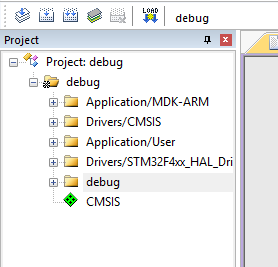
\includegraphics[width=0.6\linewidth]{module.png}
 \caption{Module hóa trong KeilC}
\end{figure}
\paragraph{}
Bạn có thể thấy trong Keil C khi mới generate từ CubeMX ra có chứa các thư mục, mỗi thư mục là một nhóm chức năng và mỗi chức năng là môt file .c khác nhau. Ngoài ra nó còn lưu đường dẫn đến cái file header .h. Bạn vào Project -> Options for Target...->C/C++ -> Include Paths, để xem các đường dẫn này.
\paragraph{}
Mình từng gặp mấy bạn mới code viết tất cả mọi thứ vào hàm main (kinh dị) từ đọc cảm biến, đọc nút nhấn, điều khiển động cơ... Bạn nên viết hoặc sử dụng thư viện cho mỗi loại phần cứng đó, rồi trong hàm main chỉ gọi hàm trong thư viện đó ra.
\paragraph{}
Một nguyên tắc để code bạn dễ đọc: trong một trang ít code thôi, và chúng liên quan tới nhau, không thể viết thư viện điều khiển động cơ và đọc nút nhấn vô chung một chỗ được.
\section{Gọi hàm từ thư viện}
\paragraph{}
Mỗi một thư viện thì thường có 2 file chính, file source code \textit{.c} và file header \textit{.h}.File \textit{.c} thì để bạn viết code trong đó rồi, còn file \textit{.h} sẽ là bảng mô tả những gì mà file \textit{.c} có thể làm, nó khai báo các hàm mà các module khác có thể gọi để sử dụng thư viện này. Hay nói cách khác thì file \textit{.h} sẽ là trung gian của giữa nơi gọi hàm và nơi thực thi hàm.
\paragraph{}
Bạn vào file main.c trong một project, ấn chuột phải vào hàm và chọn Go To Definition Of... để đến nơi hàm đó được định nghĩa (trong file .c), chọn Go To Reference To... để đến nơi hàm đó được khai báo (trong file .h).
\newpage
\section{Cấu trúc hàm main và cách gọi hàm}
\paragraph{}
Hàm main thường có cấu trúc là khởi tạo và vòn lặp chương trình chính. Tương tự như arduino nó setup() và loop().
\begin{lstlisting}
void main(void)
{
	system_init();
	
	while(1)
	{
		//Do what you want
	}
}

\end{lstlisting}
\paragraph{}
Ví dụ như mình viết một chương trình đọc cảm biến và 10 phút gửi về một lần. Thì mình sẽ viết như sau:
\begin{lstlisting}
void main(void)
{
	system_init();
	
	while(1)
	{
		read_sensor();
		send_data();
		delay(10_minutes);
	}
}
\end{lstlisting}
\paragraph{}
Bạn thấy không, chương trình mình viết nó y chang những gì mình nói. Còn việc các hàm đọc cảm biến read\_sensor() hoặc gửi dữ liệu về send\_data\_to\_master\_mcu() nó ra sao trong đó thì viết ở chỗ khác. Đừng nhét mọi thứ mà bạn có thể viết ra vào đây, làm ơn!!!
\paragraph{}
Có một khái niệm về \textbf{mức trừu tượng}. Ví dụ như hàm đọc cảm biến read\_sensor có thể bao gồm 3 hàm thế này:
\begin{lstlisting}
void read_sensor(void)
{
	request_sensor_data();
	wait_for_sensor_data();
	save_sensor_data();
}
\end{lstlisting}
đầu tiên ra lệnh cho cảm biến, sau đó chờ và khi dữ liệu về thì cất đâu đó. Bạn có thể thấy mức trừu tượng của hàm read\_sensor sẽ cao hơn 3 hàm trong đó vì nó bao hàm 3 cái hàm này. Hàm read\_sensor thì có mức trừu tượng bằng với hàm 2 hàm còn lại trong vòng while(1) của hàm main vì đây là 3 bước tuần tự nhau trong một công việc.
\paragraph{}
Nói tóm lại hãy phân thứ bậc cho các hàm (như mô hình đa cấp ấy :) và khi một hàm gọi các hàm con thì nhớ rằng các hàm con nên có cùng mức trừu tượng với nhau.
\begin{figure}[h!]
	\centering
	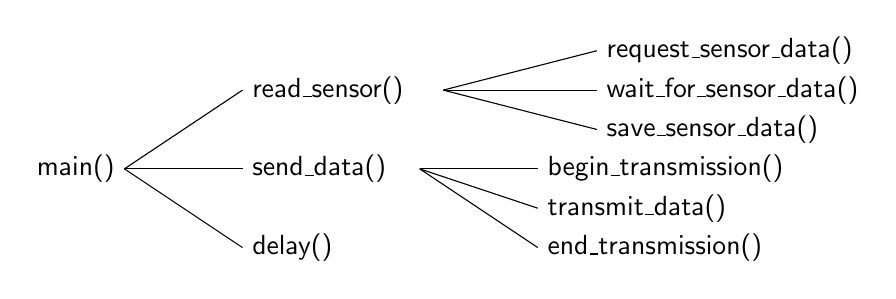
\begin{tikzpicture}[yscale=0.5, xscale=1.5]
	\node [left] at (0, 0) {main()};

	\draw (0,0) -- (1, 2);
	\node [right] at (1,2) {read\_sensor()};
		\draw (2.7,2) -- (4, 3);
		\node [right] at (4,3) {request\_sensor\_data()};
		\draw (2.7,2) -- (4, 2);
		\node [right] at (4,2) {wait\_for\_sensor\_data()};
		\draw (2.7,2) -- (4, 1);
		\node [right] at (4,1) {save\_sensor\_data()};
	\draw (0,0) -- (1, 0);
	\node [right] at (1,0) {send\_data()};
		\draw (2.5,0) -- (3.5, 0);
		\node [right] at (3.5,0) {begin\_transmission()};
		\draw (2.5,0) -- (3.5,-1);
		\node [right] at (3.5, -1) {transmit\_data()};
		\draw (2.5,0) -- (3.5, -2);
		\node [right] at (3.5, -2) {end\_transmission()};

	\draw (0,0) -- (1, -2);
	\node [right] at (1,-2) {delay()};
	
		
	\end{tikzpicture}
	\caption{Mô hình đa cấp.}
\end{figure}
\paragraph{}
Nhớ là hông phải mình làm màu mà viết tên hàm tiếng Anh đâu, vì tiếng Việt không dấu nó như teencode vậy đọc không nổi, mà nhiều khi hiểu lộn nghĩa :).
\section{Cách hàm số}
\paragraph{}
Việc phát minh ra các hàm con là phát minh vĩ đại như phát minh ra cái máy tính vậy. Nếu không có hàm con thì bạn tưởng tượng viết chương trình một lèo từ đầu tới cuối xem.
\paragraph{}
Vậy nên để đạt hiệu quả thì cần có những lưu ý sau:
\subsection{Đặt tên hàm}
\paragraph{}
Tên hàm được đặt để cho biết cái \textbf{hàm con đó nó làm cái gì}. Ví dụ như read\_sensor() chẳng hạn, dù bạn chưa biết cảm biến loại gì và đọc nó như thế nào nhưng cũng hiểu sơ sơ về mục đích gọi hàm.
\paragraph{}
Và hàm \textbf{chỉ làm những gì mà tên hàm nói đến, không hơn không kém}. Trong khi viết code thì mọi thứ nên được viết tường minh ra. Ví dụ như hàm gọi hàm send\_data() để truyền dữ liệu về, nếu khi truyền xong muốn xóa dữ liệu cũ đi thì gọi hàm delete\_data() sau khi gọi hàm send\_data().
\begin{lstlisting}
while(1)
{
	read_sensor();
	send_data();
	delete_data();
	delay(10_minutes);
}
\end{lstlisting}
Không nên nhét hàm delete\_data() vào bên trong send\_data() như muốn hiểu ngầm "gửi xong rồi xóa nó đi chứ để làm gì". Vì nhiều khi có việc cần đến nó.
\paragraph{}
Một vài ví dụ như khi viết vội có bạn đặt tên hàm kiểu ham\_a(), ham\_b(), hoặc func\_1(), func\_2(), mai mốt đọc lại xỉu.
\paragraph{}
Việc bạn đặt tên hàm rồi sau thấy củ chuối quá thì cũng đừng ngại đổi lại nhé, mình nhiều khi cũng phải đổi 2-3 lần mới được cái tên vừa ý.
\subsection{Độ dài của hàm}
\paragraph{}
Nguyên tắc để dễ code dễ đọc: code ngắn thôi, với lại tên hàm đặt đúng với yêu cầu. 
\paragraph{}
Một số hàm chỉ hoạt động tốt nếu nó đủ dài, cắt ngắn lại thành ra dở. Tuy nhiên đa số các trường hợp bạn có thể cắt một hàm dài bất tận ra thành các hàm nhỏ, như chia giai đoạn ra, rồi đặt tên hàm theo các giai đoạn của chương trình. Rất thường xuyên hàm viết ra để gọi có một lần, nó không có tác dụng là tránh lặp lại code như mục đích sinh ra hàm ban đầu, nó chỉ có tác dụng làm chương trình bạn gọn gàng hơn, dễ đọc hơn.
\paragraph{}
Còn độ dài của nó bao nhiêu là vừa. Cái này bạn phải làm rồi rút ra kinh nghiệm cho bản thân. Với mình thì dài dưới 10 dòng là okie nhất, trên 20 dòng thì nên cắt nó đi.
\subsection{Truyền tham số}
\paragraph{}
Tham số là nơi giao tiếp của hàm này với hàm kia. Mà nói chung là một hàm khai báo tham số đầu vào cũng ít thôi. Bạn viết một hàm với yêu cầu truyền 5 cái thông số đầu vào thì làm sao bạn nhớ được thứ tự của tham số đó mà truyền cho đúng?
\subsection{Bảo vệ hàm số}
\paragraph{}
Giả sử bạn viết một hàm chia a cho b như sau:
\begin{lstlisting}
float a_divide_b(int a, int b)
{
	return (float)a/b;
}
\end{lstlisting}

\paragraph{}
Rồi bỗng một ngày đẹp trời, một thanh niên lấy hàm bạn viết ra, rồi xài như sau: float result = a\_divide\_b(2, 0). Xong biên dịch thì không báo lỗi nhưng mà chạy cái nó xịt khói. Đây là lỗi chia cho 0, thành ra nó không tính được và chạy loạn xạ.
\paragraph{}
Thế nên với mỗi chương trình có truyền tham số vào, hãy nhớ là kiểm tra coi nó có hợp lệ hay không, nếu tính toán thì tham số đưa vào có thuộc tập xác định hay không... Bởi vì bạn sẽ không biết sau này người dùng hàm sẽ truyền cái gì vào trong đó nên phải kiểm tra lại. Nguyên tắc kiểm tra là : không tin cha con thằng nào cả. Đừng hi vọng họ sẽ truyền vào tham số hợp lệ, thường thì họ chả quan tâm đâu. Nên nhớ đầu vào hợp lệ thì mới thực thi hàm.
\paragraph{}
Hàm có kiểm tra tham số đầu vào:
\begin{lstlisting}
float a_divide_b(int a, int b)
{
	if(b==0){
		//printf("Divided by 0 error\n");
		return 0;
	}
	return (float)a/b;
}
\end{lstlisting}


\section{Các biến số}

\chapter{Quản lý phiên bản: GIT}
\chapter{Viết thư viện}
\chapter{Blocking vs Non-blocking}

\end{document}
